\documentclass[12pt,oneside]{book}

\usepackage{latexsym}
\usepackage[empty]{fullpage}
\usepackage{titlesec}
\usepackage{marvosym}
\usepackage[usenames,dvipsnames]{color}
\usepackage{verbatim}
\usepackage{enumitem}
\usepackage{etoolbox}





\renewcommand\bibname{ }
\usepackage{mathptmx}
\usepackage{graphicx}
\usepackage{wrapfig}
\usepackage[utf8]{inputenc}
\usepackage{fancyhdr}
 \pagestyle{fancy}
\fancyhf{}
%\lhead{Curriculum vitae}
\cfoot{ \hrule {\small Moslem Heidarpur}{\hfill\small Page \thepage ~of 5}}
 \usepackage{geometry}
 \geometry{
 a4paper,
 total={170mm,257mm},
 left=15mm,
 top=17mm,
 right=15mm,
  bottom=37mm,
 }
\setlength{\headsep}{0.2in} 
\setlength{\footskip}{0.5in} 

\newcommand{\fd}{\small \textit}
%\newcommand{\mtf}{ \fontfamily{put}\selectfont}
\newcommand{\mtf}{ \bf \normalsize}
\usepackage{array}
\newcolumntype{L}[1]{>{\raggedright\let\newline\\\arraybackslash\hspace{0pt}}m{#1}}
\newcolumntype{C}[1]{>{\centering\let\newline\\\arraybackslash\hspace{0pt}}m{#1}}
\newcolumntype{R}[1]{>{\raggedleft\let\newline\\\arraybackslash\hspace{0pt}}m{#1}}

\usepackage[resetlabels]{multibib}
\bibliographystyle{ieeetr}
%\newcites{crypto}{{dff}} 

\patchcmd{\thebibliography}{\chapter*}{\section*}{}{}

\newcites{main,crypto}{{},{}}



\begin{document}\thispagestyle{empty}
 \thispagestyle{empty}
 \lhead{Research statement}
 \phantom \quad \\

{\bf Research Statement: 
Designing efficient and high performance SOCs  Embedded system for emerging technologies
%A Neuromorphic Processor For Biological Neural Neural Networks
}
\vspace*{2\baselineskip}\\
%{\bf Background } 
Nowadays, embedded systems has became inseparable part of many modern devices. These systems include automobiles, UAVs, smart grids, wireless networks, medical devices, industrial controllers etc. With expanding to Internet Of Things (IOTs), it is expected that every device in the near future includes an embedded system. 

With expansion of usage, embedded systems face new challenges. An example is automotive section where self-driving cars require real-time processing which require very high performance embedded devices. Nevertheless, they require high levels of security, reliability and safety. Embedded systems in these modern cars also has limitation on power usage and usually must acquire various network connectivity protocols. Adding to the already long list, the resources for designing such devices is constrained and in most case, they need to be backward compatible. 


Addressing such challenges requires unconventional and novel approaches. In many applications such neural network inference engines and cryptography systems, the fetch and decode processors are incapable of keeping up with increasing demand for computational power, specially with approaching to the end of the Mooore's law. Same scenario also applies to power usage. An example of very power efficient  processing systems is human brain. A system which is intelligent, fast, fault tolerant and yet it uses fraction of the power used by Von Neumann computers. 

These research proposals aim to tackle these problems by developing non Von Neumann architectures. In this research plan, two areas where these new approaches are intended to apply are elaborated. \\
  \thispagestyle{empty}
 \lhead{Research Proposal: Post Quantum Hardware Cryptography and Homomorphic  Encryption}
 \phantom \quad \\
\hrule \phantom \quad  \vspace*{1\baselineskip}  \\
 {\bf Research Proposal: Post Quantum Hardware Cryptography and Homomorphic  Encryption}
 \vspace*{1\baselineskip}  \hrule \phantom \quad \\


\begin {itemize}
 \item [$\bullet$] { \bf Summary:} \vspace{0.5em} \\
This research program focuses on simplifying the complexity and ensuring efficient hardware implementation of post-quantum cryptography, homomorphic encryption, and homomorphic data processing embedded systems.

 \item [$\bullet$] { \bf Introduction:} \vspace{0.5em} \\
This research proposal aims to address two aspects of concern related to modern communication devices and systems. The first aspect is security, and the second aspect is privacy.
\begin{itemize}
\item [-]
Security: \\ Cryptographic systems have become integral components of nearly every communication device, providing confidentiality, data security, and authentication in various applications such as communication devices, autonomous vehicles, the Internet of Things (IoT), and healthcare [1,2,3,4]. However, the advent of quantum computers capable of executing the Shor algorithm [5] poses a threat to popular public key cryptography systems like RSA and elliptic curve cryptography. This jeopardizes the security of digital communications and exposes user data. The National Institute of Standards and Technology (NIST) has initiated a competition for developing cryptographic systems resistant to quantum computer attacks, with round 3 submissions currently underway [6].
\item [-]
Privacy: \\ Another issue arising from the expansion of the Internet and cloud systems is privacy concern. Despite secure communication between user computers and cloud systems, data is still decrypted in the cloud for processing. Consequently, third parties with access can read and exploit the data. Homomorphic Encryption (HE), introduced by Gentry, is a privacy-preserving algorithm enabling computation over encrypted data without decryption.
\end{itemize}
As these algorithms are expected to shape future cryptographic systems, designing efficient embedded systems for their implementation is crucial. In the next section, I elaborate on my methods to address this challenge.
 \item [$\bullet$] { \bf Challenges:} \vspace{0.5em} \\
 In this section, the challenges ahead of  Post-Quantum Cryptography (PQC) and Homomorphic Encryption (HE) is briefly explained and how this research proposal tries to address these challenges.
 
 
 
 Post-quantum cryptography  are believed to be secure against attacks by quantum computers.  While post-quantum cryptography aims to provide alternatives that resist quantum attacks, it also faces several challenges:
\begin{itemize}

 \item[-]   Standardization: There is not yet a widely accepted standard for post-quantum cryptographic algorithms. 
 \item[-]  Migration: Transitioning from existing cryptographic systems to post-quantum cryptography poses challenges. It requires updating protocols, systems, and infrastructure across various applications and services, which can be a time-consuming and complex process.
 \item[-]     Performance: Many post-quantum cryptographic algorithms are computationally more intensive than current algorithms, potentially leading to performance challenges, especially in resource-constrained environments. Researchers are working to optimize these algorithms to improve efficiency.
  \item[-]    Implementation Issues: Implementing cryptographic algorithms correctly is crucial for security. However, there's a risk that poorly implemented post-quantum algorithms may introduce vulnerabilities. Ensuring secure and correct implementations is a challenge, especially given the complexity of some post-quantum cryptographic schemes.
  \item[-]    Lack of Real-World Testing: Post-quantum cryptographic algorithms are relatively new, and their real-world performance and security need to be validated through extensive testing and deployment. Until these algorithms are widely deployed and tested, their effectiveness and resilience against both quantum and classical attacks remain theoretical.
  \item[-]    Quantum-Safe Key Management: Post-quantum cryptographic systems rely on key exchange mechanisms, and secure key management is crucial. Quantum-safe key exchange protocols need to be developed and integrated into existing systems to ensure that keys remain secure even in a post-quantum world.
 \item[-]     Evolving Threat Landscape: The threat landscape is dynamic, and adversaries may adapt their strategies and techniques. Post-quantum cryptographic algorithms need to be resilient not only to known quantum attacks but also to potential new attack vectors that may emerge.
  \item[-]    Global Adoption: Achieving global adoption of post-quantum cryptographic standards is a challenge. Different countries and organizations may have varying levels of readiness and priorities, and achieving a coordinated transition is essential for overall security.
 \end{itemize}
 
 
 
 
Homomorphic encryption  provides a significant advantage for privacy and security in scenarios where sensitive data needs to be processed in a secure manner. However, homomorphic decryption, or more accurately, the challenge associated with homomorphic encryption, involves several factors:
\begin{itemize}

  \item[-]   Computational Overhead: Homomorphic encryption typically introduces a significant computational overhead. Performing operations on encrypted data is computationally more intensive than on the equivalent unencrypted data. This can lead to slower processing times, making it less practical for certain applications.

 \item[-]    Key Management: Managing the keys used in homomorphic encryption is crucial. If keys are compromised, it can potentially lead to the compromise of the entire encrypted data. Key management becomes even more challenging as the complexity of the homomorphic encryption scheme increases.

 \item[-]    Limited Functionality: While homomorphic encryption allows for certain types of computations on encrypted data, it may not support all types of operations. Some computations, particularly those involving complex data structures or iterative algorithms, can be challenging to perform efficiently in a homomorphically encrypted domain.

  \item[-]   Size Expansion: Homomorphic encryption can cause significant expansion in the size of the encrypted data compared to the original unencrypted data. This can be a concern, especially when dealing with large datasets.

   \item[-]  Adaptation of Applications: Existing applications and algorithms may need to be adapted or restructured to work with homomorphic encryption. This can be a barrier to the widespread adoption of this technology.
\end{itemize}

 \item [$\bullet$] { \bf Proposed Research:} \vspace{0.5em} \\
This research objective is to develop a novel hardware-based solution aimed at addressing  challenge such as Performance, Implementation Issues, Lack of Real-World Testing, Quantum-Safe Key management. The key characteristics of the proposed encryption hardware is listed below:
\begin{itemize}
   \item[-]   Design and implement a hardware accelerator for post-quantum cryptographic algorithms to enhance performance.
   \item[-]   Address implementation challenges, ensuring robustness against side-channel attacks, fault-injection attacks, Differential Power Analysis (DPA), and Tempest Attacks.
  \item[-]    Conduct extensive real-world testing to validate the effectiveness and practicality of the proposed hardware solution.
  \item[-]    Develop quantum-safe key management protocols suitable for integration into existing cryptographic systems.
\end {itemize}
Regarding the HE, the main objective of this research would be to design a hardware capable of the performing neural network inference on the encrypted data. The hardware focus would be on efficient addition and subtraction. Leverage parallel processing capabilities and optimized memory management to enhance overall performance.The objectives of this research are:
    \begin{itemize}
    \item[-]    Break down neural network inference computations into homomorphic encryption-supported operations, emphasizing addition, subtraction, and minimizing multiplications.
  \item[-]   Design a specialized hardware accelerator targeting homomorphic encryption operations to significantly improve computational efficiency.
  \item[-]   Mitigate key management challenges associated with homomorphic encryption, ensuring secure and efficient use.
  \item[-]   Adapt the proposed hardware accelerator for seamless integration into neural network applications
    \end{itemize}
 \item [$\bullet$] { \bf Method:} \vspace{0.5em} \\
  The methodology to carry out  the PQC research proposal could be breakdown into following phases:
 \begin{itemize}
 \item [-]  Phase 1, Hardware Design and Verification: Design a specialized hardware architecture optimized for PQC encryption, focusing on enhancing performance while minimizing costs. Considerations will include parallel processing capabilities, efficient memory management, and power consumption optimization.
 \item [-]  Phase 2, Implementation Robustness: Implement countermeasures against common cryptographic attacks, including side-channel attacks, fault-injection attacks, DPA, and Tempest Attacks. Employ techniques such as secure coding practices, constant-time algorithms, and hardware-based protections to fortify the implementation against potential vulnerabilities.
  \item [-]  Phase 3, Real-World Testing:
Conduct comprehensive real-world testing in various scenarios to evaluate the proposed hardware's performance, scalability, and compatibility with existing systems. Collaborate with industry partners and organizations to simulate diverse deployment environments.
  \item [-]  Phase 4, Quantum-Safe Key Management:
Develop and implement quantum-safe key management protocols that ensure the security and integrity of cryptographic keys. Evaluate the resilience of these protocols against both classical and quantum attacks.
 \end{itemize}
 The methodology to carry out the HE research proposal could be breakdown into phases:
     \begin{itemize}
     \item [-]  Phase 1, Neural Network Optimization: Explore the methods (such as sparsity) to minimize the number of computations required to perform inference. Since, the HE computations are expensive, this phase can significantly improve the overall performance. 
     \item [-]  Phase 2, Operation Breakdown: Analyze neural network inference computations to identify opportunities for minimizing multiplicative operations. Propose strategies to restructure computations and replace multiplications with more homomorphic encryption-friendly additions and subtractions.
     \item [-] Phase 3, Implementation: This phase aims to implement the HE based neural network inference engine on hardware. In this research proposal, Field Programmable Gate Arrays (FPGAs) are chosen as the initial implementation target for their reconfigurability, affordability, and speed.
      
      \item [-] Phase 4, Verification and Testing: This phase aims to test the designed hardware and verify the functionality. The patterns are encrypted using He algorithms and would serve as inputs to test the HE based NN inference engine. The obtained accuracy should be closed to the accuracy obtained from the hardware. 
            \item [-] Phase 5, Real-world Application: Explore methods to seamlessly integrate the designed hardware accelerator into existing neural network applications. Address compatibility issues and provide adaptation guidelines to facilitate widespread adoption.
     \end{itemize}
%\item [-]
 \item [$\bullet$] { \bf Current Research:} \vspace{0.5em} \\
While working as a postdoctoral researcher at the University of Windsor, I began my research in cryptography by focusing on creating efficient hardware for multiplying binary polynomials. The results of this project were successfully published in a well-known journal.

Afterwards, I shifted my focus to Post-Quantum Cryptography (PQC) and Homomorphic Encryption (HE) algorithms. I worked on improving the efficiency of hardware for multiplying large integer polynomials, a crucial aspect in PQC and HE cryptography systems. Specifically, I addressed the challenge of slow and resource-intensive polynomial multiplication by using the Number Theoretic Transform (NTT), a widely adopted algorithm.

This work was completed during my part-time role as a researcher at the University of Windsor, resulting in the filing of a provisional patent. Currently, we are working on obtaining a patent for the developed circuit. Additionally, a circuit was developed based on this concept to perform hardware multiplication of extremely large integers for Fully Homomorphic Encryption (FHE), addressing the challenge of dealing with very large numbers. This research in under review for publication. 

Regarding the Neural Networks, where I strategically utilized sparsity to achieve a significant reduction in the number of parameters by almost 80$\%$, without compromising accuracy. This reduction substantially lowered the computation required for inference tasks. The overarching goal is to apply these techniques to reduce computational requirements when performing inference on the encrypted data using HE.
 \item [$\bullet$] { \bf Research Program Feasibility:} \vspace{0.5em} \\
 The first phase involves optimizing algorithms for hardware implementation using Python for simulations and FPGAs for efficiency measurement. FPGAs, being cost-effective and flexible, are advantageous over designing and fabricating a VLSI ASIC. After testing, the design can be fabricated for final evaluations. Three defined projects include studying post-quantum cryptographic algorithms, investigating homomorphic encryption and ciphertext computation algorithms, and designing an architecture and circuit for efficient hardware implementation.
 \item [$\bullet$] { \bf Funding and Grant Potential:} \vspace{0.5em} \\
Leveraging my industry background and familiarity with industry problems, I plan to secure funding for the research. I have successfully written research proposals with industry partners to obtain MITACS grants in the past. 
       
\begin{itemize}
\item [-]
    Natural Sciences and Engineering Research Council of Canada (NSERC):
        NSERC provides grants to support research in natural sciences and engineering, including computer science and cryptography.
%\item [-]
%    Canadian Cyber Threat Exchange (CCTX):
%        CCTX focuses on cybersecurity initiatives and may have funding opportunities for research related to cryptographic solutions and encryption technologies.

\item [-] Tech Companies:

    IBM Research: Companies like IBM have research divisions that may fund projects related to cryptography and encryption.\\
    Microsoft Research: Microsoft has an interest in various areas of cryptography and may provide research grants.
\item [-]
    Canadian Institutes of Health Research (CIHR):
        CIHR may provide funding for research projects that involve the intersection of health data and encryption technologies.
\item [-]
    Mitacs:
        Mitacs offers collaborative research internships and training programs that connect researchers with industry partners. It could be a valuable resource for projects with practical applications.
\item [-]
    Canada Foundation for Innovation (CFI):
        CFI supports state-of-the-art infrastructure for research. If your project involves the development of specialized equipment or facilities, CFI might be a relevant funding source.
%\item [-]
%    Canadian Security Establishment (CSE):
%        CSE is focused on cybersecurity and may have opportunities for collaborative research projects in the area of encryption and secure communication.
\item [-]
    Defence Research and Development Canada (DRDC):
        DRDC, as the research arm of the Canadian Department of National Defence, may fund projects related to cryptographic solutions with applications in defense and security.
%\item [-]
%    Information and Communications Technology Council (ICTC):
%        ICTC focuses on advancing Canada's digital economy and workforce. They may support research projects that contribute to the advancement of encryption technologies.
\item [-]
    Federal Economic Development Agency for Southern Ontario (FedDev):
        Ontario support academic research in emerging technologies through FedDev.
\end{itemize}

 \end {itemize}
\hspace*{-1.8em}
{\bf References} \\
%\vspace*{-4em}
{\footnotesize
\begin{itemize}
\item[] [1] J. Yoo and J. H. Yi, “Code-based authentication scheme for lightweight integrity checking of smart vehicles,” IEEE Access,
vol. 6, pp. 46731–46741, 2018.
\item[] [2] R. Abu-Salma, M. A. Sasse, J. Bonneau, A. Danilova, A. Naiakshina, and M. Smith, “Obstacles to the adoption of secure
communication tools,” in 2017 IEEE Symposium on Security and Privacy (SP), pp. 137–153, 2017.
\item[] [3] P. Aparna and P. V. V. Kishore, “Biometric-based efficient medical image watermarking in e-healthcare application,” IET
Image Processing, vol. 13, no. 3, pp. 421–428, 2019.
\item[] [4] T. D. P. Bai, K. M. Raj, and S. A. Rabara, “Elliptic curve cryptography based security framework for internet of things (iot)
enabled smart card,” in 2017 World Congress on Computing and Communication Technologies (WCCCT), pp. 43–46, 2017.
\item[] [5] P. W. Shor, "Algorithms for quantum computation: discrete logarithms and factoring," Proceedings 35th Annual Symposium on Foundations of Computer Science, 1994, pp. 124-134, doi: 10.1109/SFCS.1994.365700
\item[] [6] “Post-Quantum Cryptography-Round 3 Submissions,” 2024.
\end{itemize}


}


%\end{itemize}


%{\bf Case II: 
%Post Quantum Hardware Cryptography and Homomorphic  Encryption}\\
%%\vspace*{3\baselineskip}\\
%This research program involves reducing complexity and efficient hardware implementation of the post quantum cryptography, homomorphic encryption, and homomorphic data processing embedded systems. \\[0.2cm]
%{\bf Background:  } 
%Cryptography systems have become  inseparable parts of almost every communication device.
%Cryptography is  used to provide confidentiality, data security, and authentication in many applications such as
%communication devices, autonomous vehicles, Internet of Things (IoT), healthcare [1,2,3,4] etc.


%However, with rise of the quantum computers capable of executing Shor algorithm  [5], many popular public key cryptography systems including RSA  and elliptic curve cryptography will be no longer secure.  This would greatly endanger the security of digital communications and expose user's data. 
% National Institute of Standards and Technology (NIST) has already started a competition for developing cryptographic systems that are resistant to quantum computers attacks. At present, NIST has called for submissions for round 3 of this completion [6]. 
%%The submission for previous rounds could be find in references \citecrypto{nistr2,nistr1}. 


%Another issue with expansion of the Internet and cloud systems is privacy concern. 
% Currently, with the most secure communication between user computer and cloud system, still the data is decrypted in the cloud for processing. Therefore, the third parties owning the cloud and those with authorized access can read the data and use it for their own advantages. Homomorphic Encryption (HE), first introduced by Gentry  is a privacy preserving algorithm that allows valid computing over encrypted data without the need to decrypting it. 
% 
% Since these algorithms are expected to be the future  cryptography systems, it is important to design an efficient  embedded systems for these systems. In next section,
% I further explain my methods to address this challenge. \\
%{\bf Method: } 
%Since  post quantum cryptography is a rather new field and because of  complexity of its algorithms, there exists only a limited number of the hardware implementations for these algorithms. 
% In this research proposal, Field Programmable Gate Arrays is selected as the initial implementation target since they provide a  reconfigurable, cheap and yet fast hardware platform. 
% % Round 3  finalists for public-key encryption, key establishment and digital signature are already available in NIST website. Most of these algorithms come only with a software implementation. Even those with hardware implementation still have plenty of room for improvement. This also applies to homomorphic encryption and computation as I discuss it further in the following. 
%  In homomorphic encryption, plaintext is transformed into ciphertext, allowing computation on the encrypted data resulting in another ciphertext. Decryption of this ciphertext yields the same computation result as if it had been performed on plaintext.
% % \begin{figure}
%% \centering
%%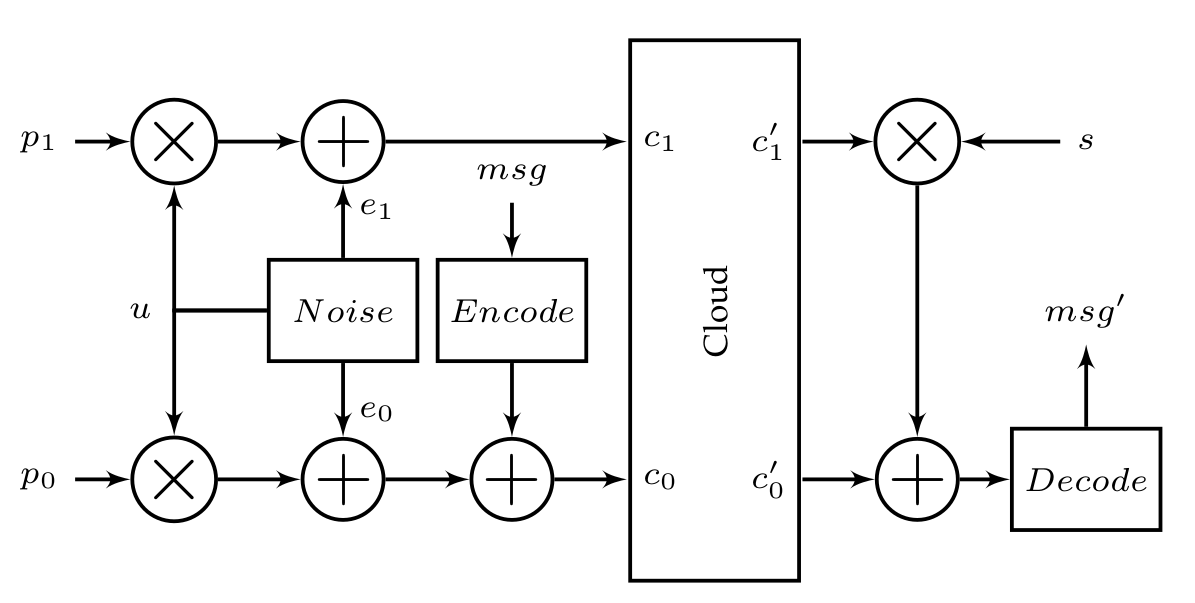
\includegraphics[scale=0.18]{fv.png}
%%  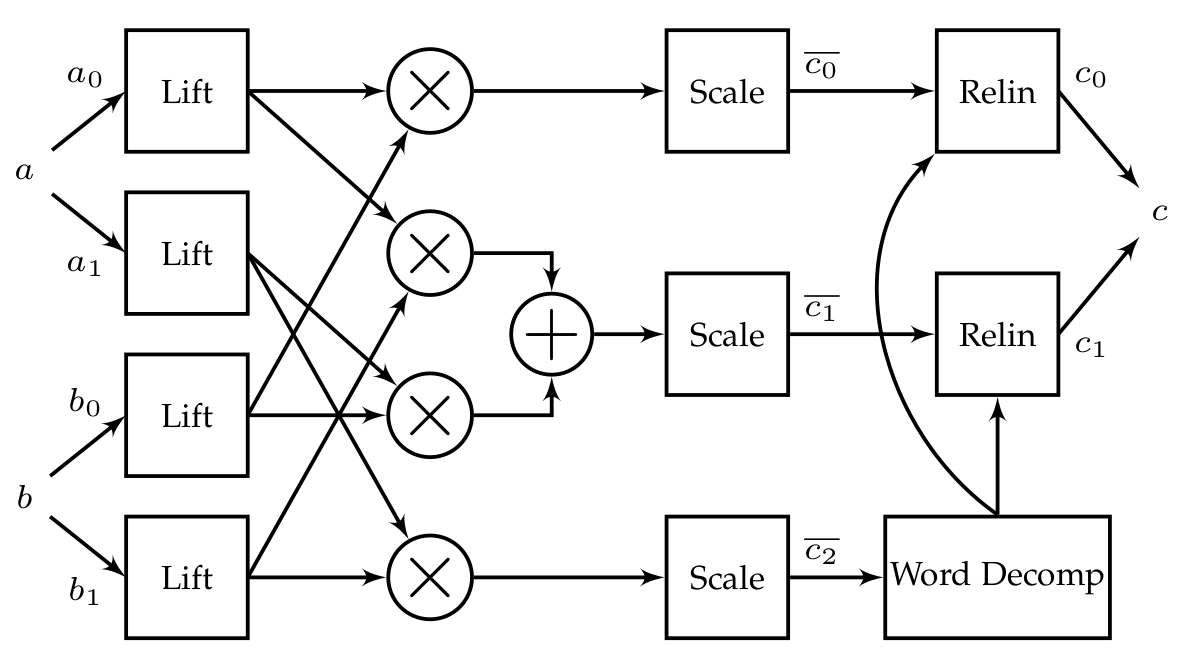
\includegraphics[scale=0.18]{fvhom.png}\\[-0.5em]
%%(a)\hspace{7.2cm}(b)
%%  \caption{(a) Fan and Vercauteren  (FV) encryption  encrypts a message into pair of ciphertexts c0 and c1 using public keys p0 and p1. 
%%  (b) Fan and Vercauteren homomorphic multiplication over the ciphertexts (figures are taken from \cite{turan2020heaws}.)}
%%  \label{hom}
%% \end{figure}
%% HE is based on lattice problems and adds noise during encryption. The value of this noise becomes greater each time an operation is performed on the ciphertext. 
%% Somewhat Homomorphic  Encryption (SHE) scheme only allows limited number of the operations on the ciphertext and more than that, the signal to noise ratio becomes so large that the original data could not be recovered anymore. Gentry in his paper introduced use of bootstrapping technique which is basically homomorphic evaluation of
%%the decryption circuit in the cloud to refresh and remove extra noises.
%% This resulted into Fully Homomorphic  Encryption (FHE). 
% However, such  operations are computationally expensive and increases the complexity of the homomorphic  computations circuit. 
%% Fig. \ref{hom} shows the circuit for homomorphic  encryption and homomorphic multiplication over encrypted data for  FV \citecrypto{fv} scheme. 
% Compared to software implementations, hardware cryptography results in a higher speed and a lower cost, while satisfying efficiency and low-power requirements of electronic
%devices. Implementation of homomorphic encryption and evaluation circuit is a extremely challenging because of the very large word length of ciphertexts and computational unit, specifically multipliers. Homomorphic encryption  is a rather new research topic and its hardware implementation is less explored. In the following, I discuss my approach towards this  problem to achieve a better hardware for practical homomorphic encryption and data processing. 
%%First, is studying the homomorphic encryption and computation to reduce their complexity and optimize them for hardware implementation. For instance, polynomial multiplication is 
%%one of  the operations that is frequently performed over very large size operands (eg. 4096 coefficients of 180-bit size  ) and plays a key role in overall performance and cost of the hardware. Therefore, it is  important to optimize these algorithm as much as possible before implementing on hardware. 
%%Second, is designing and efficient hardware architecture to encrypt and process data homomorphically. \\[0.2cm]
%\\{\bf Previous Research: }
%As postdoctoral fellow, I was working on the efficient  FPGA implementation of  finite field multipliers for Elliptic Curve Cryptography (ECC)  where we proposed a new binary polynomial multiplication algorithm with low complexity and high speed.
%The work was then extended to to hardware implementation of lattice based cryptography  algorithms and other post-quantum encryption algorithms.
%\\
%% Currently, I am closely monitoring PhD students researching in post quantum cryptography and homomorphic encryption where their research is focused on designing an FPGA based embedded processor for these algorithms.  \\
%{\bf Future Research (Research Plan): }
%My future research plan engages both studying and optimizing post quantum and homomorphic  encryption  and computation algorithms as well as designing an efficient embedded processor and processor for these algorithms. 
%%Towards this objectives, I defined 3 projects.\\[0.2cm]
%%{\bf Project 1}
%%
%%This project aims to study the different algorithms presented by researchers for 
%%post quantum cryptography including finalists of the NIST completion to standardize  quantum resistant public key cryptographic algorithms. The objective of this study is to reduce complexity and optimize these algorithms for FPGA implementation. 
%%\\[0.2cm]
%%{\bf Project 2}
%%
%%Investigating homomorphic encryption and ciphertext computation algorithms. Students will 
%%perform mathematical analysis to enhance these algorithm in the terms of area and delay complexity. Further, they will run computer simulations to check validity of the algorithms. 
%%\\[0.2cm]
%%{\bf Project 3}
%%
%%Students will design an architecture and circuit to efficiently implement  these algorithms on hardware, either as accelerator for computer software or possibly as an standalone hardware cryptography system.\\[0.2cm]
%\\{\bf Research Program Feasibility: }
%For the first phase which is optimizing  algorithms for hardware implementation, I will use Python programming language to run simulations and check the validity of  modified algorithms.  Further, I will use FPGAs as implementation platform to measure efficiency of design. FPGAs are substantially cheaper than designing  and fabricating a VLSI ASIC and have advantage of flexibility. Eventually, after testing design could be fabricated for final evaluations. Towards this objectives, I defined 3 projects:
% Project 1: 
%This project aims to study the different algorithms presented by researchers for 
%post quantum cryptography including finalists of the NIST completion to standardize  quantum resistant public key cryptographic algorithms. The objective of this study is to reduce complexity and optimize these algorithms for FPGA implementation. 
%{ Project 2:}
%Investigating homomorphic encryption and ciphertext computation algorithms. Students will 
%perform mathematical analysis to enhance these algorithm in the terms of area and delay complexity. Further, they will run computer simulations to check validity of the algorithms. 
%{ Project 3:}
%Students will design an architecture and circuit to efficiently implement  these algorithms on hardware, either as accelerator for computer software or possibly as an standalone hardware cryptography system.
%\\{\bf Funding for research }
%In terms of funding , I would be able to use my background and familiarity with problems and concerns of industry to secure funding for the research. I have also experience of writing successful research proposal with industry partner to obtain MITACS grant. \\ 
%\hspace*{-1.8em}
%{\bf References} \\
%%\vspace*{-4em}
%{\footnotesize
%\phantom \quad [1] J. Yoo and J. H. Yi, “Code-based authentication scheme for lightweight integrity checking of smart vehicles,” IEEE Access,
%vol. 6, pp. 46731–46741, 2018.\\[-0.1em]
%\phantom \quad [2] R. Abu-Salma, M. A. Sasse, J. Bonneau, A. Danilova, A. Naiakshina, and M. Smith, “Obstacles to the adoption of secure
%communication tools,” in 2017 IEEE Symposium on Security and Privacy (SP), pp. 137–153, 2017.\\[-0.1em]
%\phantom \quad [3] P. Aparna and P. V. V. Kishore, “Biometric-based efficient medical image watermarking in e-healthcare application,” IET
%Image Processing, vol. 13, no. 3, pp. 421–428, 2019.\\[-0.1em]
%\phantom \quad [4] T. D. P. Bai, K. M. Raj, and S. A. Rabara, “Elliptic curve cryptography based security framework for internet of things (iot)
%enabled smart card,” in 2017 World Congress on Computing and Communication Technologies (WCCCT), pp. 43–46, 2017.\\[-0.1em]
%\phantom \quad [5] P. W. Shor, "Algorithms for quantum computation: discrete logarithms and factoring," Proceedings 35th Annual Symposium on Foundations of Computer Science, 1994, pp. 124-134, doi: 10.1109/SFCS.1994.365700\\[-0.1em]
%\phantom \quad [6] “Post-Quantum Cryptography-Round 3 Submissions,” 2020.

%}

  \thispagestyle{empty}
 \lhead{Research Proposal: A biologically inspired neuromorphic processor}
 \phantom \quad \\
\hrule \phantom \quad  \vspace*{1\baselineskip}  \\
 {\bf Research Proposal: A biologically inspired neuromorphic processor}
 \vspace*{1\baselineskip}  \hrule \phantom \quad \\


\begin {itemize}

 \item [$\bullet$] { \bf Summary:} \vspace{0.5em} \\
This research program will engage  students in studying learning algorithms for biological neural network as well as designing innovative high-performance, low-area and power-efficient  and  biologically plausible embedded neuromorphic processors.

 \item [$\bullet$] { \bf Introduction:} \vspace{0.5em} \\
A Spiking Neural Network (SNN) is a type of artificial neural network inspired by the way biological neurons communicate in the brain. Unlike conventional neural networks, which are based on the concept of continuous activation values (e.g., in feedforward or recurrent neural networks with sigmoid or rectified linear unit activations), SNNs model the information processing in terms of discrete spikes, or action potentials. The information is encoded in the temporal domain,  taking into account the  timing and rate of the firing of action potentials. Overall, SNNs are faster and more energy efficient comparing to conventional neural networks [1,2].  



Neuromorphic systems  include a large number of spiking neurons, synapses and their interconnecting structure on hardware.  Such systems are highly parallel, fast, fault tolerant,  intelligent and compact. Further, Neuromorphic systems often operate in an event-driven manner, processing information only when there is a change or event in the input, rather than continuously processing static data. This event-driven approach can lead to increased energy efficiency.  This research focus is on neuromorphic systems implementing Spiking Neural Networks (SNNs). 
 \item [$\bullet$] { \bf Challenges:} \vspace{0.5em} \\
Implementing Spiking Neural Networks (SNNs) poses several challenges, both in terms of hardware and software aspects. In the following, some of these challenges are outlined. 
\begin{itemize}
\item[-] Training Complexity: Training SNNs is more challenging compared to conventional neural networks. The discrete and temporal nature of spikes makes it difficult to apply traditional backpropagation algorithms directly. Developing effective and efficient training algorithms for SNNs, 
is an active area of research.
\item [-] Sparse Connectivity: In biological neural networks, connectivity between neurons is often sparse. Implementing and optimizing sparse connectivity efficiently in hardware poses challenges.
\item[-] Temporal Precision: The temporal dynamics of SNNs play a crucial role in information processing. Achieving high temporal precision in hardware implementations is challenging, especially in the presence of noise and variability.
\item[-] Energy Efficiency: While SNNs are expected to be more energy-efficient than traditional neural networks, achieving this efficiency in hardware implementation requires specialized architectures. Developing low-power neuromorphic hardware that can efficiently handle spiking dynamics is a significant challenge.
\item[-] Real-Time Processing: SNNs are well-suited for real-time processing, but achieving low-latency implementations on hardware platforms is a challenge. This is particularly important for applications such as robotics and sensor networks
\end{itemize}

The objective of this research is to contribute to advancements in neuromorphic hardware, novel training algorithms, and dedicated hardware frameworks to help overcome some of the limitations associated with the implementation of neuromorphic systems.
\item [$\bullet$] { \bf Proposed Research:} \vspace{0.5em} \\
This research proposal aims to address these challenges by designing and implementing a neuromorphic hardware platform on FPGA (Field-Programmable Gate Array). The primary objectives include the design of a hardware architecture optimized for SNNs on FPGA, development of hardware-friendly training algorithms, addressing challenges related to temporal precision and real-time processing, and achieving energy-efficient spiking neural processing.
 \item [$\bullet$] { \bf Method:} \vspace{0.5em} \\
   The methodology to carry out this the PQC research proposal could be breakdown into following phases:
   \begin{itemize}
   
  \item[-] Phase 1, Training Algorithm: This phase focuses on optimizing training algorithms suitable for hardware acceleration, with a focus on the temporal dynamics of SNNs .Spike-timing-dependent plasticity (STDP) is a popular learning rule observed in the synapses of biological neural networks. It refers to the phenomenon where the strength of a synaptic connection between two neurons is modified based on the relative timing of their spikes (action potentials). STDP is a form of Hebbian plasticity, a concept derived from Donald Hebb's hypothesis that states "cells that fire together wire together."
  The STDP rule can be summarized as follows:
        \begin{itemize}
       \item [] If a presynaptic neuron fires shortly before a postsynaptic neuron, the synaptic strength is potentiated (increased).
       \item[]  If a postsynaptic neuron fires shortly before a presynaptic neuron, the synaptic strength is depressed (decreased).
        \end{itemize}
       At end of this phase, an optimized version of STDP is developed and its learning capabilities are validated through simulations and experiments  
       This research aims to use novel methods such as Time To First Spike (TTFS) to ehance the speed and energy efficiency of the neuromprhic hardware. TTFS refers to the time it takes for a neuron to generate its first action potential (spike) in response to a specific input stimulus. TTFS can modulate the learning window of STDP, allowing neurons with shorter TTFS to contribute more to synaptic potentiation. During unsupervised learning, neurons that respond quickly (short TTFS) to specific patterns in the input data can have their connections strengthened, enhancing their sensitivity to those patterns. Regarding the inference, neurons with shorter TTFS may be preferentially assigned to represent specific features or patterns in the input data, leading to a form of spike-based coding. Therefore, applying TTFS could considerably improve the inference time comparing to the rate coding in SNNs. Furthermore, it would also contribute to reducing power consumption.
       
Another methods would be utilized in this research is to optimize the neuromorphic system is sparsity. 
There are two main aspects of sparsity in SNNs:
    \begin{itemize}
    \item[]   Sparse Connectivity:
    In a sparsely connected network, each neuron typically receives input from only a subset of the neurons in the previous layer. This sparse connectivity is thought to be more biologically realistic, as not all neurons in the brain are connected to every other neuron.
    \item[]   Sparse Activity:
    Sparse activity refers to the fact that at any given time, only a small fraction of neurons in the network are active or "spiking." Most neurons remain inactive, and only a few neurons produce spikes in response to specific stimuli.
    \end{itemize}
Using sparsity contribute considerably to improve the neuromorphic hardware performance and efficiency. Some of the advantages of Sparsity in SNNs are listed below:
    \begin{itemize}
        \item[] Energy Efficiency:
        Sparse connectivity and activity contribute to energy efficiency. In a sparse network, fewer connections need to be updated, reducing the overall energy consumption during information processing. This is particularly important in neuromorphic computing, where mimicking the brain's energy-efficient processing is a goal.
        \item[] Computation Efficiency:
        Sparse connectivity reduces the computational load on the network. During information propagation, only a fraction of neurons need to be updated, leading to more efficient computations.
        \item[]    Noise Robustness:
        Sparse networks tend to be more robust to noise. The presence of sparse activity allows the network to focus on relevant information while ignoring irrelevant or noisy input. 
        \item[]
        Facilitates Learning:
        Sparse connectivity and activity can facilitate the  Spike-Timing-Dependent Plasticity (STDP) leraning, which relies on the precise timing of spikes between connected neurons.
    \end{itemize}  
In summary, sparsity in SNNs is advantageous for achieving more biologically plausible, energy-efficient, and computationally efficient neural network models. Combining sparsity with TTFS could considerably improve the existing neuromorphic platfroms. 
\item[-] Phase 2, Hardware Design and Optimization:  In this research proposal, Field Programmable Gate Arrays (FPGAs) are chosen as the initial implementation target for their reconfigurability, affordability, and speed.
This phase will involve the design and optimization of a detailed hardware architecture  for SNNs, considering FPGA constraints and capabilitie. The designed hardware would be implemented  using hardware description languages (e.g., Verilog or VHDL) on FPGA. 
          using hardware description languages (e.g., Verilog or VHDL) for FPGA implementation. Training algorithms suitable for hardware acceleration will be implemented and optimized.
          \item [-]  Real-Time Processing Optimization: This phase mostly involve investigating methods to optimize the hardware to minimize processing delays and achieve real-time performance. Accuracy of neuromorphic system should also be evaluated and  methods to enhance temporal precision in spike communication and processing on the FPGA need to be investigated. 
           \item [-] Energy Efficiency Evaluation: At this phase, experiments are designed  to measure and evaluate the energy efficiency of the implemented neuromorphic hardware. Although FPGAs are not optimized for minimum power consumption,  at very first step the energy efficiency of the FPGA-based solution could be compared to state-of-the-art FPGA neuromorphic implementation. Some methods such as clock gating could be utilized to improve the power consumption. 
            \item [$\bullet$] { \bf Current Research:} \vspace{0.5em} \\
I started my research in neuromorphic engineering during my M.Sc. dissertation titled "Digital Implementation of a Simple Model for Astrocyte Calcium Oscillations." In this project, I made a biological astrocyte work on hardware using a technique called Piecewise Linear (PWL) approximation. After that, I explored spiking neural networks and neuromorphic engineering.

As a Ph.D. student, I used the COordinate Rotation DIgital Computer (CORDIC) method to set up the Izhikevich neuron and online spike time-dependent plasticity on hardware [5]. I chose CORDIC because it's good at calculating tricky stuff precisely and works well in hardware, unlike other methods like PWL.In another project, I made a digital version of a realistic astrocyte and glutamate-release mechanism. The hardware I designed could handle complex calculations precisely and had decent performance. This is important because simulating realistic models with lots of details using high-level models takes a long time and needs a lot of computer power. This hardware is helpful for mimicking the tripartite synapse and its parts.
           
  Throughout my time as part-time research associate at University of Windsor,  a method was presenting for reducing power consumption in an artificial neural network, the method comprising: receiving an input signal; modulating a sampling frequency of an artificial neuron based on the input signal; and forwarding the input signal or a further input signal obtained from the input signal to the artificial neuron at the sampling frequency. 
A US patent was obtained for the proposed method  [6]. 

In another work, Selective Input Sparsity (SIS) method proposed for edge inference applications in image classification where the image acquisition environment is controlled. These sparsely connected networks are well-suited to area-constrained applications as they require fewer neurons and synapses than baseline Fully Connected (FC) networks of analogous structures. The SIS networks require fewer hardware resources and make inferences faster than the baseline FC networks without substantial impact on the classification accuracy [7].
 \item [$\bullet$] { \bf Research Program Feasibility:} \vspace{0.5em} \\
The research project comprises four key phases. The initial phase involves studying algorithms and optimization techniques for neuromorphic hardware. This phase is conducted without the need for specialized equipment and is primarily planned to be simulated using the Python programming language. The next phase focuses on designing and implementing the hardware, with a primary emphasis on verifying functionality. FPGAs are employed during this stage for implementation, allowing for the validation of functionality and the measurement of design efficiency. In the third phase, FPGAs are also used in optimizing performance to meet Real-Time Processing requirements. In the final stage, the emphasis shifts towards ASIC (Application-Specific Integrated Circuit) implementation. While an initial evaluation can be performed on FPGAs, it is noteworthy that FPGAs are not inherently power-efficient devices
\item [$\bullet$] { \bf Funding and Grant Potential:} 
Leveraging my industry background and familiarity with industry problems, I plan to secure funding for the research. I have successfully written research proposals with industry partners to obtain MITACS grants in the past. 
 \begin {itemize}
    \item [-]  Natural Sciences and Engineering Research Council of Canada (NSERC):
    NSERC is a federal agency that provides funding for research in natural sciences and engineering. Their Discovery Grants program may support 
    projects related to neuromorphic engineering.
    \item [-] Tech Companies:
    \begin {itemize}
    \item []   IBM Research:
         IBM has a significant interest in neuromorphic computing and artificial intelligence. IBM Research may provide funding for projects aligned with their neuromorphic computing research objectives.
    \item [] Intel Labs:
        Intel is actively involved in research and development in neuromorphic computing. This may provide funding opportunities through Intel Labs, particularly in areas related to hardware and architecture.
    \item []   Google Research:
        Google has a strong focus on artificial intelligence and machine learning. Google Research may offer funding or collaborative opportunities for projects related to neuromorphic engineering and SNNs.
    \item [] NVIDIA:
        NVIDIA is a key player in the graphics processing unit (GPU) market and has been involved in AI research. They may support research projects that leverage GPU technology for neuromorphic applications
\end {itemize}
 \item [-] Canadian Institutes of Health Research (CIHR):
    CIHR focuses on health-related research, and certain programs within CIHR may support studies that involve neural networks and brain-related technologies.
\item [-]     Canada Foundation for Innovation (CFI):
    CFI provides funding for research infrastructure.While working on neuromorphic engineering projects, I may be abe to receive support for acquiring or upgrading relevant equipment and facilities.
 \item [-] Mitacs:
   \item [-]  Mitacs  collaborate with academia, industry, and government, and their programs may be applicable to research in neuromorphic engineering.
  \item [-]   National Research Council Canada (NRC):
    NRC is the Government of Canada's research organization. Collaborative projects related to neuromorphic engineering may find support through various NRC programs.
    \item [-]
    Federal Economic Development Agency for Southern Ontario (FedDev):
        Ontario support academic research in emerging technologies through FedDev.
         \end {itemize}
   \end{itemize}






%are faster, smaller in size, more energy efficient and biologically realistic [1,2]. 

% Implementation of SNNs is computationally expensive because of
%nonlinear expressions in neuron models, size of the networks
%and various communication pathways.
%% A simplified  biological neuron with its corresponding connections is shown in Fig. \ref{bneuron}. A neuron could be connected to hundreds of the  other cells including neurons and astrocytes.    
% This research objective is to address this challenges by designing efficient and high speed hardware implementation platform for SNN.
\end {itemize}

\hspace*{-1em}
{\bf References} \\
%\vspace*{-4em}
{\footnotesize
\begin {itemize}
\item [] 1] K. E. Friedl, A. R. Voelker, A. Peer, and C. Eliasmith, “Human-inspired neurorobotic system for classifying surface textures
by touch,” IEEE Robotics and Automation Letters, vol. 1, no. 1, pp. 516–523, 2016.
\item [] [2] F. Ponulak and A. Kasinski, "Introduction to spiking neural networks: Information processing, learning and applications.,"
Acta neurobiologiae experimentalis, vol. 71, no. 4, pp. 409-433, 2011.
\item [] [3]  Brzosko, Z., Mierau, S.B. and Paulsen, O., 2019. Neuromodulation of spike-timing-dependent plasticity: past, present, and future. Neuron, 103(4), pp.563-581.
\item [] [4] Rueckauer, B. and Liu, S.C., 2018, May. Conversion of analog to spiking neural networks using sparse temporal coding. In 2018 IEEE international symposium on circuits and systems (ISCAS) (pp. 1-5).
\item [] [4] M. Heidarpur, A. Ahmadi, M. Ahmadi and M. Rahimi Azghadi, "CORDIC-SNN: On-FPGA STDP Learning With Izhikevich Neurons," in IEEE Transactions on Circuits and Systems I: Regular Papers, vol. 66, no. 7, pp. 2651-2661, July 2019
\item [] [5] Mirhassani, M., Heidarpur, M. and Leigh, A.J., University Of Windsor, 2023. Dual State Circuit for Energy Efficient Hardware Implementation of Spiking Neural Networks. U.S. Patent Application 17/984,612.
\item [] [6] A. J. Leigh, M. Heidarpur and M. Mirhassani, "Digital Hardware Implementations of Spiking Neural Networks With Selective Input Sparsity for Edge Inferences in Controlled Image Acquisition Environments," in IEEE Transactions on Circuits and Systems II: Express Briefs, vol. 70, no. 5, pp. 1724-1728, May 2023
\end {itemize}
%\phantom \quad [1] K. E. Friedl, A. R. Voelker, A. Peer, and C. Eliasmith, “Human-inspired neurorobotic system for classifying surface textures
%by touch,” IEEE Robotics and Automation Letters, vol. 1, no. 1, pp. 516–523, 2016.\\[-0.1em]
%\phantom \quad [2] F. Ponulak and A. Kasinski, "Introduction to spiking neural networks: Information processing, learning and applications.,"
%Acta neurobiologiae experimentalis, vol. 71, no. 4, pp. 409-433, 2011.\\[-0.1em]
%\phantom \quad [3]  Brzosko, Z., Mierau, S.B. and Paulsen, O., 2019. Neuromodulation of spike-timing-dependent plasticity: past, present, and future. Neuron, 103(4), pp.563-581.\\[-0.1em]
%\phantom \quad [4] Rueckauer, B. and Liu, S.C., 2018, May. Conversion of analog to spiking neural networks using sparse temporal coding. In 2018 IEEE international symposium on circuits and systems (ISCAS) (pp. 1-5).\\[-0.1em]
%%\phantom \quad [3] M. Samie, G. Dragffy, A. M. Tyrrell, T. Pipe, and P. Bremner, “Novel bio-inspired approach for fault-tolerant vlsi systems,”
%IEEE Transactions on Very Large Scale Integration (VLSI) Systems, vol. 21, no. 10, pp. 1878–1891, 2013.\\[-0.1em]
%\phantom \quad [4] A. L. Hodgkin and A. F. Huxley, “A quantitative description of membrane current and its application to conduction and
%excitation in nerve,” The Journal of physiology, vol. 117, no. 4, p. 500, 1952.\\[-0.1em]
%\phantom \quad [5] E. M. Izhikevich, “Simple model of spiking neurons,” IEEE Transactions on neural networks, vol. 14, no. 6, pp. 1569–1572,
%2003.
}




%{\bf Case I: A biologically inspired neuromorphic processor: } \\
%This research program will engage  students in studying learning algorithms for biological neural network as well as designing innovative high-performance, low-area and power-efficient  and  biologically plausible embedded neuromorphic processors.\\ [0.2cm]
%{\bf Background: } 
%%Over the past decades, researchers have been trying to 
%%emulate and study the brain for both medical and information processing applications. Some medical objectives include understanding neurological and psychiatric diseases \cite{capecci2015feasibility}, 
%%simulation of drug treatment \cite{wallach2015atomnet} as well as designing brain computer interfaces for people with sensory, motor and cognitive
%%disabilities \cite{li2016collaborative}. Nevertheless, brain study is more important
%%from an information processing point of view. The analysis of
%%the brain's information processing mechanism can eventually lead to a new
%%generation of computational devices  that are expected to be
%%intelligent, power efficient and fast \cite{7378880,6145692}. Contrary to current
%%computers, brain inspired systems will be more tolerant to both
%%hardware and data failures \cite{6376255}.
%%
%%\begin{wrapfigure}{l}{0.5\textwidth}
%%\centering
%%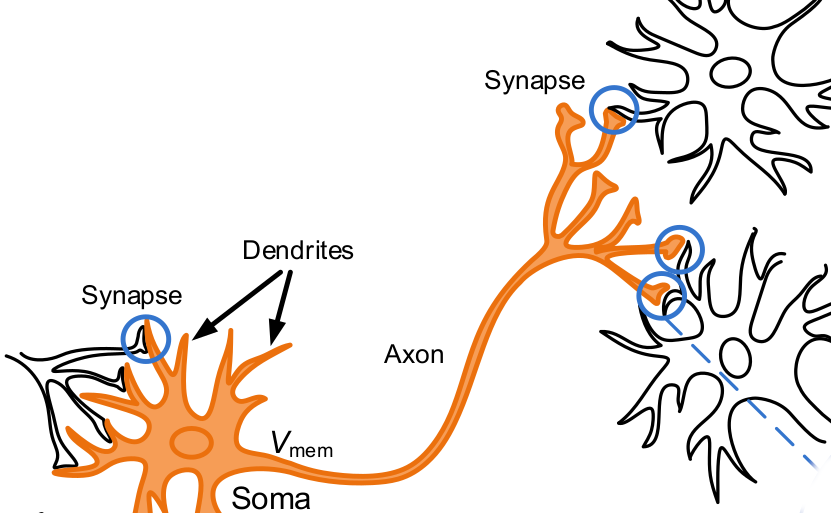
\includegraphics[scale=0.21]{neuron.png}
%%\caption{Simplified diagram of a typical biological neural cell \cite{wu2015cmos}.}
%%\label{bneuron}
%%\end{wrapfigure}

%A Spiking Neural Network (SNN) is a type of artificial neural network inspired by the way biological neurons communicate in the brain. Unlike conventional neural networks, which are based on the concept of continuous activation values (e.g., in feedforward or recurrent neural networks with sigmoid or rectified linear unit activations), SNNs model the information processing in terms of discrete spikes, or action potentials. The information is encoded in the temporal domain,  taking into account the  timing and rate of the firing of action potentials. Overall, SNNs are faster and more energy efficient comparing to conventional neural networks.  

%Neuromorphic systems  include a large number of neurons, synapses and their interconnecting structure on hardware.  Such systems are highly parallel, fast, fault tolerant,  intelligent and compact.  This research focus is on neuromorphic systems implementing Spiking Neural Networks (SNNs). 
%Spiking neural networks  are the third generation of neural networks where neurons communicate through sparse sequences of spikes. Comparing to previous generations, SNNs
%are faster, smaller in size, more energy efficient and biologically realistic [1,2]. 

% Implementation of SNNs is computationally expensive because of
%nonlinear expressions in neuron models, size of the networks
%and various communication pathways.
%% A simplified  biological neuron with its corresponding connections is shown in Fig. \ref{bneuron}. A neuron could be connected to hundreds of the  other cells including neurons and astrocytes.    
% This research objective is to address this challenges by designing efficient and high speed hardware implementation platform for SNN.
%\\ [0.2cm]
%{\bf Methods: }
%%
%%One approach to study   biological neural networks is to divide it into two
%%hierarchical sub-levels of components and architecture. The
%%components level, representing the lowest level of abstraction,
%%involves studying and mathematically modeling the properties
%%and interactions of cells within the network. The architectural level,
%%however, deals with the complex interactional behaviors of
%%a large number of inter-connected components. Activities that
%%occur at the architectural level include learning and 
%%information processing in the biological neural networks. 
%%
%%At the cell level, this research has two objectives; First, is analyzing the cells  differential equation and performing bifurcation analysis  to  optimize these  ODEs for a high-performance and low-cost    implementation. Second, is designing efficient circuits for hardware implementation of these cells. These two objectives are clarified further in the following.
%%
%%
%Current neuromorphic research has led to the development of a plethora of models to mimic real neurons with different levels of abstraction in biological details [3,4]. 
%%Biologically-plausible models such as Hodgkin Huxley \cite{hodgkin1952quantitative}
%%describe cellular phenomena and properties of the individual
%%biological components. Such low-level models impose more
%%computation cost, making it difficult to simulate large-scale
%%networks. On the other hand, biologically-inspired models
%%such as Izhikevich \cite{izhikevich2003simple}, aim to
%%mimic the biological neurons to the best degree of accuracy.
%%Such models can reproduce most of the firing patterns of real
%%neurons and are easier to couple to other spike-oriented units.
%%Moreover, high-level Integrate and Fire (IF) \cite{gerstner2002spiking} is another
%%computationally efficient neuron model, but it cannot exhibit
%%many essential features of the biological neurons as observed
%%in experiments. 
%The choice of models depends
%on the application of the device to be designed. 
%%To perform
%%computations with SNNs only a simple IF or Exponential
%%IF (EIF) may be enough to act as a thresholding box.
%%However, for research in neuroscience, biologically plausible
%%models have higher flexibility in mimicking biology.
% In this research we intend to focus on
%biologically plausible and detailed models and optimize them without comprising their  correctness.  

% %Second objective at cell level is designing practical circuits realizing these cells using hardware implementation techniques (e.g.
%  First objective at the lowest  level is designing practical circuits realizing brain cells using hardware implementation techniques (e.g. pipelining and power optimization techniques).  It is very important to implement the cell
%models as efficient and fast as possible since they are basic building block of the neuromorphic systems. 
%Biologically plausible models are  relatively complex in nature comparing to high-level models due to their large array of differential equations and accompanying parameters.
%As a result, they have  seen limited
%proposed hardware implementations. Currently, there is no neuromorphic processor available for large scale simulation of the biologically detailed models. 
% However these models are gaining
%more attention by researchers. 


%At the architectural and software levels, brain cells are connected together through different interaction mechanisms and their systematic behavior is analyzed. 
%%T
%%his is useful to study biological functions and disorders as well as discovering computational algorithms underlying information processing, learning and memory in the brain. 
%This research has two objectives in architectural level; First is applying brain inspired learning and information processing algorithms in the software level and second is  designing a configurable hardware for large scale implementation of biological neural network. \\
%%In the following,  I will explain these two objectives in more details. 
%%
%%
%%
%%The exact mechanism of information processing and learning algorithm in the brain is yet unknown. However, 
%%Spike Timing Dependent Plasticity (STDP) is the most popular method  for unsupervised online training of 
%%feed-forward  biological neural networks. This method is based on Hebbian learning where analogous to biology, the synaptic weight changes when a pre-synaptic neuron fires
%%in a short time before or after the post-synaptic neuron,
%%strengthening or weakening the neuron connection accordingly. Such a change is determined as an exponential of the time difference between two events. 
%%
%%Large scale hardware implementation of biological neural networks could be divided into two steps. First steps is implement nonlinear bio-chemical reactions between components and second  is to design an architecture to implement  various communication pathways. 
%%\\ [0.2cm]
%{\bf Previous Research: } 
%My M.Sc. dissertation titled ``Digital Implementation of a Concise Model for Astrocyte Calcium Oscillations" was beginning of my research in the field of neuromorphic engineering where I optimized a biological astrocyte for hardware implementation using Piece Wise Linear (PWL) approximation technique. Since, I continued to research in spiking neural network and neuromorphic engineering. As a PhD student, I started using COordinate Rotation DIgital Computer (CORDIC) method to implement Izhikevch neuron and on-hardware online spike time dependent plasticity.  The advantage of CORDIC algorithm over previous methods including PWL, is its very high precision to calculate nonlinear terms and yet it is well suited for hardware implementation.  
%%In another work, a  digital implementation of a biologically plausible astrocyte and glutamate-release mechanism was presented.  
%% The designed hardware was capable of calculating nonlinear functions with a very
%%high precision while having relatively high performance. This is most important because, unlike high level models, simulation of biologically plausible models 
%%due to high biological details requires long time and computational
%%power and will fall behind the real time easily. This hardware is
%%most useful to emulate the tripartite synapse and its components.
%The primary goal of those researches was to find an appropriate hardware for neurons, astrocytes and other biological cells as buildings blocks of a biological detailed neuromorphic processor.\\
%{\bf Future Research }\\
%My future research plan involves
% both studying  algorithms underlying learning and information processing in biological neural network as well 
% designing neuromorphic processor for large scale implementation of such networks. 
%% Towards this objectives, I defined 4 projects. \\ [0.2cm]
%%{\bf Project 1} 
%%
%%This project aims  to study the different models presented by researchers to mimic biological cells that are involved in information processing in the brain. The objective is to adapt and modify differential equation describing these models to maximize performance and minimize power consumption and area. Students will run computer simulation of these models and perform bifurcation analysis to look for possible modification or approximation in these models.
%%\\ [0.2cm]
%%{\bf Project 2} 
%%
%%Designing digital circuits for ODEs describing cells. Students will use hardware implementation and optimization techniques to increase performance and reduce power consumption and area of  designs. The circuits need to be simulated to ensure their validity. 
%%\\  [0.2cm]
%%{\bf Project 3} 
%%
%%Studying interactions of the cells within the biological neural networks and investigate the mechanisms behind  learning, information processing and 
%%energy efficiency. Students will run computer simulations to observe changing of biological parameters and ions concentrations inside and around the cells that are active in learning and information processing.   
%%\\  [0.2cm]
%%{\bf Project 4} 
%%
%%Large scale implementation of the biological cells and   communication pathways in the biology. Students will design a new architecture capable of online on-chip learning with  biological neural networks. \\[0.2cm]
%%%-------------------
%%{\bf Research Program Feasibility} 
%%
%%\begin{wrapfigure}{l}{0.5\textwidth}
%%\centering
%%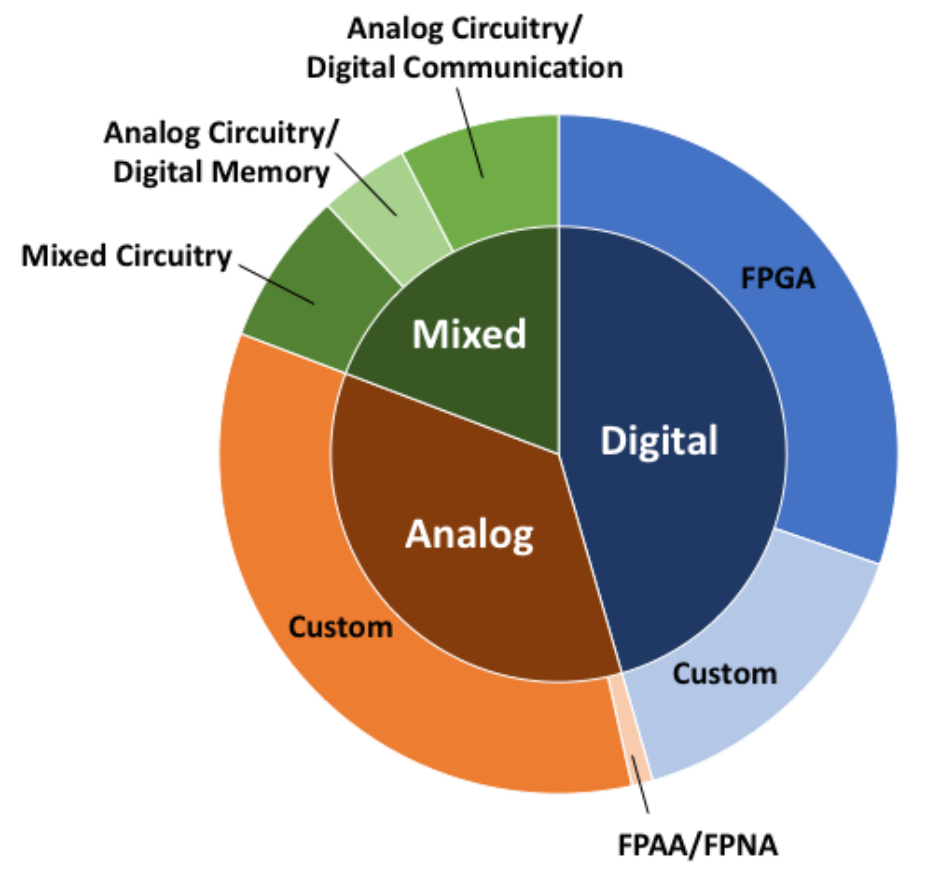
\includegraphics[scale=0.18]{hardware.png}
%%\caption{An overview of hardware implementations in neuromorphic computing \cite{schuman2017survey}.}
%%\label{fpga}
%%\end{wrapfigure}
%%The research would be initially computational, it can be  performed at a small
%%undergraduate institution. 
%Design prototypes would be implemented and tested on Field Programmable Gate Arrays (FPGAs) at first phase. FPGAs provide relatively cheap, fast, reconfigurable, and easy to work with platform for testing functionality and performance of the digital hardwares and are a popular implementation platform
% %as shown in Fig. \ref{fpga}.
%  Second phase is designing an Application Specified Integrated Circuit (ASIC)  to implement the neuromorphic processor which require softwares such Cadence that currently are accessible   through CMC Microelectronics for universities. Finally, the design need to be fabricated that is also is supported by CMC Microelectronics.
%  The primary goal of those researches was to find an appropriate hardware for neurons, astrocytes and other biological cells as buildings blocks of a biological detailed neuromorphic processor.\\
%{\bf Future Research  }\\
%My future research plan involves both studying  algorithms underlying learning and information processing in biological neural network as well designing neuromorphic processor for large scale implementation of such networks. Towards these objectives, I defined 4 projects. \\ 
%{ Project 1:} 
%This project aims  to study the different models presented by researchers . The objective is to adapt and modify differential equation describing these models to maximize performance and minimize power consumption and area. Students will run computer simulation of these models.
%{ Project 2:} Designing digital circuits for ODEs describing cells. Students will use hardware implementation and optimization techniques to increase performance and reduce power consumption and area of  designs. 
%{ Project 3:} 
%Students will run computer simulations to observe changing of biological parameters and ions concentrations inside and around the cells that are active in learning and information processing.   
%{ Project 4:} 
%Large scale implementation of the biological cells and   communication pathways in the biology. Students will design a new architecture capable of online on-chip learning with  biological neural networks. 
%{ Project 5:} software design and optimization for the hardware.
%  \\
%\hspace*{-1em}
%{\bf References} \\
%%\vspace*{-4em}
%{\footnotesize
%\phantom \quad [1] K. E. Friedl, A. R. Voelker, A. Peer, and C. Eliasmith, “Human-inspired neurorobotic system for classifying surface textures
%by touch,” IEEE Robotics and Automation Letters, vol. 1, no. 1, pp. 516–523, 2016.\\[-0.1em]
%\phantom \quad [2] F. Ponulak and A. Kasinski, "Introduction to spiking neural networks: Information processing, learning and applications.,"
%Acta neurobiologiae experimentalis, vol. 71, no. 4, pp. 409-433, 2011.\\[-0.1em]
%\phantom \quad [3] M. Samie, G. Dragffy, A. M. Tyrrell, T. Pipe, and P. Bremner, “Novel bio-inspired approach for fault-tolerant vlsi systems,”
%IEEE Transactions on Very Large Scale Integration (VLSI) Systems, vol. 21, no. 10, pp. 1878–1891, 2013.\\[-0.1em]
%\phantom \quad [4] A. L. Hodgkin and A. F. Huxley, “A quantitative description of membrane current and its application to conduction and
%excitation in nerve,” The Journal of physiology, vol. 117, no. 4, p. 500, 1952.\\[-0.1em]
%\phantom \quad [5] E. M. Izhikevich, “Simple model of spiking neurons,” IEEE Transactions on neural networks, vol. 14, no. 6, pp. 1569–1572,
%2003.
%}
%%\newpage
% \thispagestyle{empty}
% %\lhead{Research statement}
% \phantom \quad \\

 \end{document}
